\subsection{L1 D Cache}

The L1 D cache takes requests from LSQ and store buffer, and will exchange coherence traffic with L2 cache.

\subsubsection{Interface}

\begin{figure}
\begin{lstlisting}[caption={}]
typedef struct {
  idT id;
  Addr addr;
  Msi toState;
  MemOp op;
  ByteEn byteEn;
  Data data;
  AmoInst amoInst;
} ProcRq#(type idT) deriving(Bits, Eq, FShow);
interface L1ProcReq#(type idT);
  method Action req(ProcRq#(idT) r);
endinterface
interface L1ProcResp#(type idT);
  method Action respLd(idT id, Data resp);
  method Action respLrScAmo(idT id, Data resp);
  method ActionValue#(Tuple2#(LineByteEn, Line)) respSt(idT id);
  method Action evict(LineAddr a);
endinterface
interface DCoCache;
  interface L1ProcReq#(DProcReqId) procReq;
  method Action resetLinkAddr;
  interface Perf#(L1DPerfType) perf;
  interface ChildCacheToParent#(L1Way, void) to_parent;
  interface Get#(L1DCRqStuck) cRqStuck;
  interface Get#(L1DPRqStuck) pRqStuck;
endinterface
module mkDCoCache#(L1ProcResp#(DProcReqId) procResp)(DCoCache);
  // implementation
endmodule
\end{lstlisting}
\caption{Interface of L1 D cache}\label{fig:d-cache-ifc}
\end{figure}

Figure~\ref{fig:d-cache-ifc} shows the interface of D cache.
Struct \code{ProcRq} is the request sent to D cache from the core.
It contains the following fields:
\begin{itemize}
    \item Field \code{id}: is the ID of the request, which is the LQ index or the SB index.
    \item Field \code{addr}: is the physical address of the request.
    \item Field \code{toState}: is the minimum MESI state that is required to process the request for its cache line.
    \item Field \code{op}: is the operation of the request, i.e., load, store, load-reserve, store-conditional, or atomic memory operation (AMO).
    \item Field \code{byteEn}: is valid only for store-conditionals.
    It specifies the bytes to modify in a 8B-aligned data, i.e., \code{byteEn} has been shifted according to the lower bits of the address.
    \item Field \code{data}: is valid only for store-conditionals or AMOs.
    For store-conditionals, it is the 8B-aligned data corresponding to \code{byteEn}, i.e., it has been shifted according to the lower bits of the address..
    For AMOs, it is the data read from the source register, i.e., it is NOT shifted according to address.
    \item Field \code{amoInst}: carries more information about the AMO computation, e.g., fetch-and-add, swap, etc.
\end{itemize}
The \code{DCoCache} interface of the D cache contains the following fields:
\begin{itemize}
    \item Subinterface \code{procReq}: contains a \code{req} method which is called to send new requests to D cache.
    \item Method \code{resetLinkAddr}: clears the reservation made by load-reserves.
    This can be called when the commit stage is processing an exception or interrupt.
    \item Subinterface \code{to\_parent}: contains FIFOs to be connected to the parent L2 cache.
    \item Subinterface \code{perf}: is for querying performance counters in D cache.
    \item Subinterfaces \code{cRqStuck} and \code{pRqStuck}: are for reporting deadlocks for core requests and parent requests, respectively.
\end{itemize}
The \code{L1ProcResp} interface is passed to D cache as an argument.
Its methods will be called when the cache has acquired sufficient MESI state for the cache line to complete the request.
It contains the following fields:
\begin{itemize}
    \item Method \code{respLd}: is to respond a load request with ID \code{id}.
    Argument \code{data} is the 8B-aligned loaded data.
    We still need to shift the data before writing to register file.
    \item Method \code{respLrScAmo}: is to respond a load-reserve or store-conditional or AMO with ID \code{id}.
    In case of a load-reserve, argument \code{data} is the 8B-aligned loaded data, which needs to be shifted before being written back to register file.
    In case of a store-conditional, \code{data} indicates whether the store-conditional succeeds or not (0 means success while 1 means failure).
    In case of an AMO, \code{data} is the original memory value, which can be written back to register file without extra shifting.
    \item Method \code{respSt}: is to respond a store request with ID \code{id}.
    The return value of this method contains the bytes to be modified in the cache line, and the D cache will use this information to update the cache contents.
    \item Method \code{evict}: is called by the D cache when a cache line is evicted (by replacement or invalidation).
    This is needed only in TSO to notify LSQ that some speculative loads may need to be squashed.
\end{itemize}

\noindent\textbf{Conflict Matrix:}
All methods of interface \code{DCocCache} should be conflict free.

\subsubsection{Implementation}

\begin{figure}[t]
    \centering
    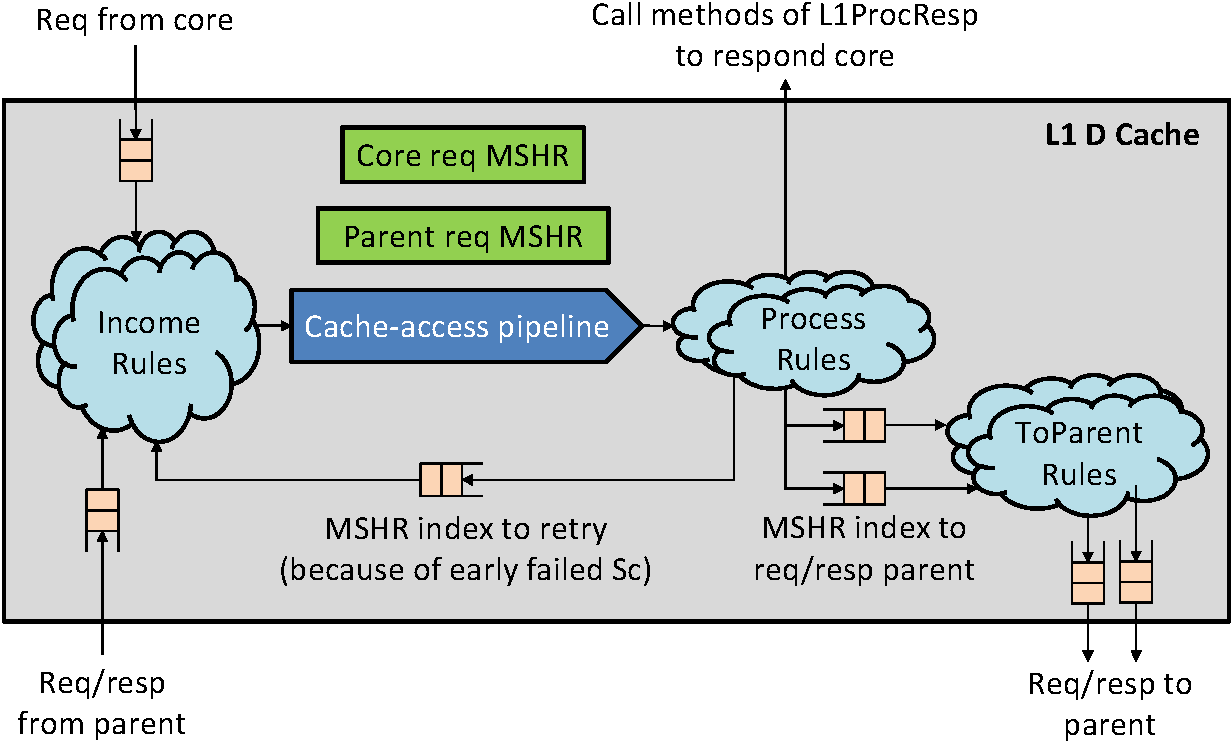
\includegraphics[width=\columnwidth]{fig/d_cache_crop.pdf}
    \caption{Internal implementation of D cache (the names of rules and submodules are different from those in source code)}\label{fig:d-cache-impl}
\end{figure}

Figure~\ref{fig:d-cache-impl} shows the internal implementation of the D cache.
It contains three submodules:
\begin{itemize}
    \item Cache-access pipeline: is a pipeline to access the cache arrays.
    It contains the following three stages:
    \begin{enumerate}
        \item Request tag SRAM.
        \item Get tag SRAM responses, perform tag matching, and request data SRAM.
        \item Get data SRAM responses, and update both data and tag SRAMs.
    \end{enumerate}
    The first and the last stages are interface methods of this submodule, which will be called by the top-level rules of the D cache.
    There are internal bypassing logic in the pipeline to resolve read-after-write hazards.
    \item MSHR for core requests: contains bookkeepings for all the in-flight requests from the core.
    \item MSHR for parent requests: contains bookkeepings for all the in-flight (downgrade) requests from the parent L2 cache.
\end{itemize}

Now we explain how the D cache functions.
Every income message from the core or the parent L2 is entered into the cache-access pipeline by an Income rule.
New requests also need to allocate MSHR entries in these rules.
At the end of the cache-access pipeline, the message is processed by a Process rule.
The Process rule will update states in the MSRH entry and tag/data SRAMs.
In case the rule finds a core request is ready to respond, it will call methods of the \code{L1ProcResp} interface to respond the core.
In case the rule needs to send messages to the parent L2, it will first enter the MSHR index of the request that needs to message L2 into a FIFO, which has the same number of entries as the MSHR and can always be enqueued.
Then the MSHR index will be picked up by a ToParent rule which truly sends a message to L2.

In our coherence protocol, core requests for the same cache line cannot be processed together; they have to be processed one by one.
To ensure this invariant, the core-request MSHR will organize requests for the same cache line as a linked list, and only the head of the list can be truly processed at the Process rule.
When the heading request is responded at the Process rule, it is removed from the MSHR, and the next request in the linked list will be directly swapped into the end of the cache-access pipeline and will be processed by the Process rule.
This increases the throughput if the core keeps requesting on the same cache line.

There is one exception to the above swapping optimization.
If the heading request is a store-conditional and it fails because the cache line is not in the D cache, then we cannot swap the next request into the end of the pipeline.
In this case, we wake up the next request, and let it go through the pipeline.

\subsubsection{Future Improvement}
The current implementation keeps requests for the same cache line in the MSHR.
However, MSHR is a critical resource, and we might want to keep only missing requests in MSHR, instead of those that are idling and waiting for others to complete.

\subsubsection{Source Code}
See the followings:
\begin{itemize}
    \item module \code{mkDCoCache} in \code{//procs/lib/L1CoCache.bsv}, and
    \item module \code{mkL1Bank} in \code{//coherence/src/L1Bank.bsv}.
\end{itemize}
